\documentclass{beamer}

\usetheme{Rochester}
\usecolortheme{material}
\usepackage{multicol}
\usepackage{listings}

\setbeamertemplate{footline}[text line]{%
  \parbox{0.5\linewidth}{
    \vspace*{-12pt} %\insertshorttitle~(\insertshortauthor)
  }
  \hfill%
  \parbox{0.5\linewidth}{
    \vspace*{-12pt}\raggedleft\insertpagenumber
  }
}
\lstset{
breaklines=true, 
basicstyle=\scriptsize, 
keywordstyle=\color{blue700},
basewidth=0.55em
}
\setbeamertemplate{navigation symbols}{}
\begin{document}
\title[Entwurssprachen]{HW/SW Codesign LU - FLAC Decoder}
\author[Platzer M., Zaruba F., Weber T.]{Michael Platzer, Florian Zaruba, Thomas Weber}
\date{\today}

\begin{frame}
\titlepage
\end{frame}

\begin{frame}\frametitle{Table of contents}
%\begin{multicols}{2}
  \tableofcontents
%\end{multicols}
\end{frame}

\section{Partitioning} 
\begin{frame}\frametitle{Partitioning} 
Ideas for the Implementation
\begin{itemize}
	\item SD-Card read in HW
	\item Display and FFT in HW
	\item ... TBA
	\item Optimizations in C code (loop unrolling,..)
\end{itemize}
\end{frame}

\section{SDCard}
\begin{frame}\frametitle{SDCard}
	
\end{frame}
\begin{frame}\frametitle{RA - Overview}
    \begin{figure}[hp]
      \centering
      \includegraphics[width=0.6\textwidth]{pictures/read_ahead_overview}
      \caption{Read-ahead overview}
      \label{fig:fft_display_struct}
    \end{figure}
\end{frame}

\begin{frame}\frametitle{RA - Buffer}
    \begin{figure}[hp]
      \centering
      \includegraphics[width=0.7\textwidth]{pictures/read_ahead_gatter}
      \caption{Read-ahead RTL}
      \label{fig:fft_display_struct}
    \end{figure}
\end{frame}

\section{FFT - Display}
\begin{frame}\frametitle{FFT-Display}
    \begin{figure}[hp]
      \centering
      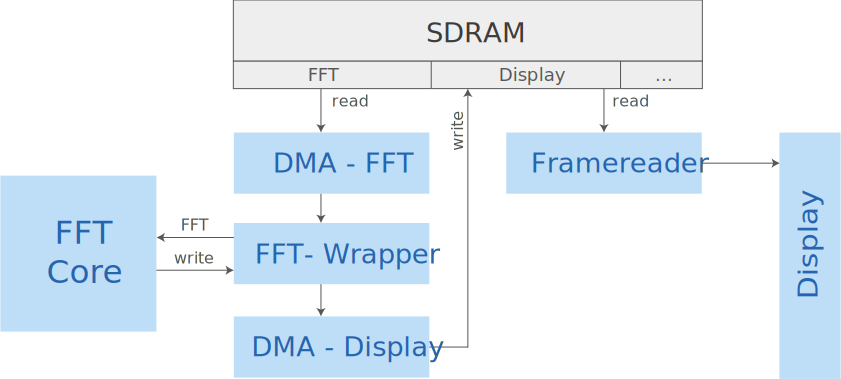
\includegraphics[width=0.9\textwidth]{pictures/fft_display}
      \caption{FFT Display overview}
      \label{fig:fft_display_struct}
    \end{figure}
\end{frame}
\section{Software}
\begin{frame}\frametitle{Software}
	
\end{frame}

\section{Problems}
\begin{frame}\frametitle{Problems}
\begin{itemize}
	\item {TBA} 
	\item {TBA}
	\item {TBA}
	\item {TBA}
\end{itemize}
\end{frame}
      
\section{Bibliography}
%\nocite{haubelt2010digitale}
%\nocite{canis2011legup}
%\nocite{liao2002system}
%\nocite{initiative2014functional}
\begin{frame}[allowframebreaks] \frametitle{Literature} 
\bibliographystyle{plain}
\bibliography{references}
\end{frame}



\end{document}
